Project Manager - Logan

\section{Process}
The initial planning of our language took place during in-person
meetings where we were able to discuss and critique ideas quickly and
effectively. We explored the differences between and application and a
language and as a result were able to eliminate many of our ideas. We
eventually narrowed our scope down to focusing on
parallelization. After getting constructive feedback on our white
paper we realized that our scope was too broad for the amount of time
we had to complete the project. We then decided to narrow this scope
down to parallelization around data manipulation, specifically in
arrays.
\subsection{Weekly Meetings}
Through out the course of the project, we have held weekly in-person
meets on Fridays. This was an opportunity for the group to check in
and make sure everyone was on the same page. After an hour or so
everyone would break up and work on their respective tasks for that
week while still allowing for collaboration.
\subsection{Github}
GitHub became an invaluable resource to the group as a shared
repository and version control. In addition, we used the GitHub issues
and milestones features to set goals for when certain parts should be
completed.  Issues allowed us to post tasks and problems that can be
assigned to an individual or multiple people. It then easily allows us
to see what is left to do and what has been accomplished already. This
allowed us to have a scheduling system that was directly tied to our
repository and stay on track.
\subsection{Google Apps}
While working remotely, we used gmail and gchat extensively for
communication. Google Calendar and docs were also used for meeting
planning and drafting the various required papers throughout the
semester.
\subsection{Testing}
We created tests at each stage of development to ensure that our work
was correct and that we could proceed without causing problems in the
next stage.

\section{Roles and Responsibilities}
The assigned roles for the group are:
\begin{itemize}
\item Logan Donovan – Project Manager
\item Sid Nair – Language Guru
\item Justin Hines – System Architect
\item Nathan Hwang - System Integrator
\item Andrew Hitti	- System Tester
\end{itemize}

While all of the positions come with specific tasks assigned to them,
each member of the group was able to contribute to the high-level
design of the language.  From there each person became responsible for
a specific portion of the project and then received help from other
group member as needed. Nathan worked on the parser and abstract
syntax tree creation. Andrew and Justin built the semantic analysis
and code generation. Sid was responsible for parallelization in
Scala. Logan wrote the sample programs and served as the primary
coordinator between individuals to help make sure everyone was working
together. In addition she wrote a good deal of the original type
checking system, which was later replaced with a more efficient model
and no longer, appears in our code. Despite these roles, all groups'
members participated in a great deal of cross-collaboration.

\section{Style Sheet}
\begin{itemize}
\item Two spaces as indentation 
\item File names and values use \_ underscores
\item Functions use lowercaseUppercase word concatentaion 
\end{itemize}

We used an OCAML Style guide that can be found at:
\\ \verb=http://caml.inria.fr/resources/doc/guides/guidelines.en.html=

A latex style sheet was also created to allow members to function
independently. It is available on the GitHub repository.
\newline
A latex style sheet was also created to allow members to function independently. It is available on the GitHub repository.
\section{Timeline and Project Log}
\begin{description}
\item{February 22} - White Paper Due
\item{March 21} - Language Reference Manual and Language Tutorial Due
\item{March 30} - Front End Completed
\item{April 13} - Basic Backend
\item{April 27} - Finished Backend + Array Implementation
\item{May 6} - Parallelization
\end{description}
These dates indicate basica completion but may not include all bug
fixes as many were discovered through further development.  \\ We had
weekly meetings on Fridays for at least 2 hours starting on February
24th.  The best way to see the actual process and the work done is to
look at the issues log. That can be found at:
\begin{verbatim}
https://github.com/sidnair09/DotPar
\end{verbatim} 
\subsection{Contribution Graphs}
\begin{figure}[H]
\centering
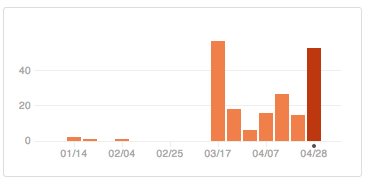
\includegraphics[scale=.5]{history.png}
\caption{A graph showing the commit history of the project over the
  course of the semester.}
\end{figure}

\begin{figure}[H]
\centering
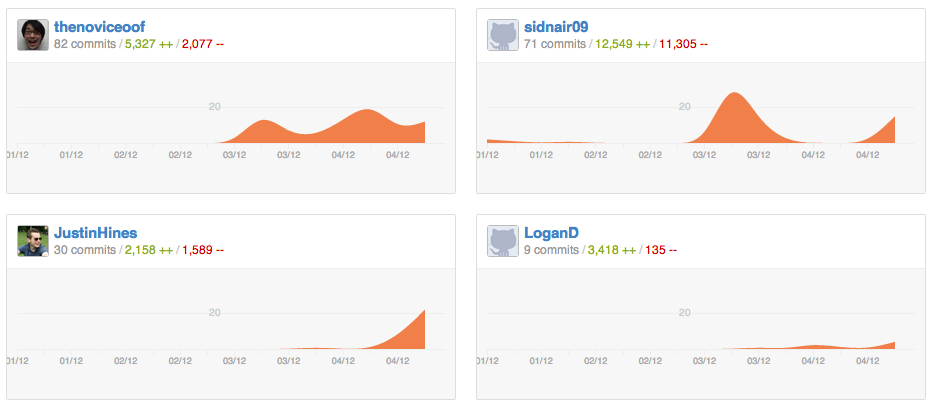
\includegraphics[width=\textwidth]{Contribution.png}
\caption{Diagram of Contributions to the Project. thenoviceof is
  Nathan, sidnair09 is Sid, JustinHines is Justin and Andrew since
  their pair program together and LoganD is Logan.}
\end{figure}
